\chapter{Interviews}
\label{ch:interviews}
\setcounter{footnote}{0}
For triangulation the defined \glspl{attribute} (\cref{sub:attributesofantifragile}) are validated by conducting interviews. The main concern for the interviews is to get an understanding of the state of \gls{antifragility} and \acrlong{ea} in the Dutch \gls{ps}. We selected interviewees from the Dutch \gls{ps} sector with a different profile than the expert group. The different profile helped with the triangulation of the research. We used \glspl{cxo} for the interviews to get the business perspective of the Dutch \gls{ps}. Four C-level Executives of the \gls{ps} participated in the interviews (\cref{tab:Interviewees}). We used a set of topics for discussion. These topics were \gls{ea}, \gls{agility}, \gls{uncertainty}, unexpected events, risk appetite, \gls{diversity} and \gls{optionality}. We expected to cover all the attributes using the topics.  The interviews were limited to an hour due to time constraints on the agenda's of the interviewees.
\begin{table}[H]
	\centering
	\resizebox{\textwidth}{!}{%
		\begin{tabular}{p{.15\textwidth}p{.85\textwidth}}
			\toprule
			\textbf{Interviewee} & \textbf{Role} \\%
			\midrule
			1 & A \acrlong{cio} from the Central Government \\%
			2 & A \acrlong{cto} from the Local Government \\%
			3 & A \acrlong{ceo} from an \acrlong{isv} \\%
			4 & A \acrlong{coo} from a Service Provider \\%
			\bottomrule
		\end{tabular}
	}%
	\caption[Interviewees]{Interviewees}%
	\label{tab:Interviewees}%
\end{table}
It was not possible to talk in-depth on \acrlong{ea}. The in-depth knowledge on the workings on \gls{ea} were less available with the interviewees. Instead of analysing the separate \glspl{attribute} of \acrlong{ea}, the analysis was on the \acrlong{ea} schools of thought \parencite{Lapalme2012}. The attributes are implicitly part of that particular school of thought.

We presented the case to the \glspl{cxo} as short as possible before we started talking about our topics. We started with a topic on \acrlong{ea}. We were particular interested in how \acrlong{ea} was practised in the organisations of the \glspl{cxo}. The rest of the topics were on the Dutch \gls{ps} in general. How \gls{agile} is the Dutch \gls{ps}, how fast can de Dutch \gls{ps} adapt to changes in the environment? Are there mechanisms in place to learn and improve? Other topics were on the Dutch \gls{ps} handles \gls{uncertainty}. Does the Dutch \gls{ps} embraces the \gls{uncertainty} or are they mitigating it? How is the Dutch \gls{ps} dealing with unexpected events. How many risks does the Dutch \gls{ps} wants to take? How diverse is the Dutch \gls{ps} and does the Dutch \gls{ps} has options to choose from? We ended the interview with subjects that we missed and possible other ideas the interviewees had on mind. We used a standard format to guide us (\cref{tab:interviewquestions})

The interviewees all wished to remain anonymous. Because of this, the transcriptions, recordings and the \gls{qda} files are not publicly available\footnote{The Antwerp Management School can request the recordings and transcriptions only for (re)accreditations and visitations to enable the Antwerp Management School to comply with statutory obligations. The recordings and transcriptions are kept for seven years after graduation before they are deleted.}. All the interviewees gave consent to transcriptions and recordings for this research.  Instead of sharing the transcriptions and recordings, this thesis contains summaries of the interviews (\cref{app:interviewsummaries}). The interviewees validated these summaries, and gave their consent to publish those instead.
\begin{table}[H]
	\centering
	\resizebox{\textwidth}{!}{%
		\begin{tabular}{@{}p{0.1\textwidth}p{0.75\textwidth}p{0.15\textwidth}@{}}
			\toprule
			\textbf{Number} & \textbf{Question} & \textbf{Concept} \\ \midrule %
			1a. & How is your organisation applying \acrshort{ea}? & \acrshort{ea} \\%
			1b. & Who is accountable for \acrshort{ea} in your organisation? & \acrshort{ea} \\%
			1c. & How is \acrshort{ea} enabling your organisation to quickly adapt to changes (external influences)? & \acrshort{ea} \\%
			2a. & Does the operational model of the\gls{ps} \gls{foster} \gls{agility}? & \Gls{antifragile} \\%
			2b. & How is the \acrshort{ea} of your organisation contributing to \gls{foster} \gls{agility} in the \gls{ps}? & \acrshort{ea} \\%
			3a. & How does the public sector deal with \gls{uncertainty}? & \Gls{antifragile} \\%
			3b. & How is the \acrshort{ea} of your organisation contributing to dealing with \gls{uncertainty} in the \gls{ps}?
			& \acrshort{ea} \\%
			4a. & How is the public sector dealing with unexpected events? & \Gls{antifragile} \\%
			4b. & How is \acrshort{ea} of your organisation contributing to dealing with unexpected events in the \gls{ps}? & \acrshort{ea} \\%
			5a. & Could you describe the risk appetite of the \gls{ps}? & \Gls{antifragile} \\%
			5b. & How does the \acrshort{ea} of your organisation match the risk appetite of the \gls{ps}?
			& \acrshort{ea} \\%
			6a. & How is \gls{diversity} and \gls{optionality} used in the \gls{ps}? & \Gls{antifragile} \\%
			6b. & How does \acrshort{ea} of your organisation support \gls{diversity} and \gls{optionality} in the \gls{ps}? & \acrshort{ea} \\%																								
			Closing & Did you miss an important subject or do you want to add something else? & non-specific \\%
			\bottomrule
		\end{tabular}
	}%
		\caption[Interview questions]{Interview questions}
		\label{tab:interviewquestions}
\end{table}
\section{Interview results}
\label{sec:interviewresults}
We could not use the raw output of the interviews for validation and analysis. It was all text. It was not directly comparable between the interviewees and with the \glspl{attribute}. We transformed these results into information that we could analyse and validate. We used \acrlong{qda} for this. We created labels to code the text of the transcriptions. For every attribute, we had two labels. We created a label for when the attribute is identified in the Dutch \gls{ps} and one for when it was not identified, but the interviewee indicated that it is necessary for the Dutch \gls{ps}. For the \gls{ea} schools of thought, we had only one label per school. A school does exist or not. Whenever we suspected to have identified a new attribute, we created the labels accordingly. The result of this analysis is available as a data set in a publicly accessible GitHub repository\footnote{\url{https://github.com/JRBliekendaal/master-thesis/blob/57f1489c59832d4c94d8bd6726d4e260f8ad544e/datasets/interviews/raw_interview_data_and_charts.xlsx}}.  

We added graphs to accompany the interpretations. These graphs support our findings. The first graph is about the \textit{frequency of an \gls{attribute}}. The second graph shows us \textit{the \% of cases (interviews)} where an \gls{attribute} occurs. The interpretation was done on the categories \gls{attenuatevariety}, \gls{amplifyvariety}, learning organisation, the \acrlong{ea} schools of thought, and the newly found \glspl{attribute}. For each of those categories we will present the results and the interpretation of the results. If applicable we use examples from the interviews to support the interpretations.
\subsection{Interview results on attenuate variety}
\label{sub:interviewresultsattenuate}
The frequency of the attributes \textit{\gls{topdowncc}} and \textit{\gls{micromanagement}} scored the highest (\cref{fig:interviewattenuatevariety}). All four interviewees mentioned both \glspl{attribute} (100\% of the cases). During the interviews, the interviewees explained that most of the sub-systems of the \gls{ps} have a severe risk-avoiding attitude. Everything must be predefined and planned because of public accountability. There is a quick result in crises, but with possible consequences later on because of \acrfull{bit} audits or \glspl{parliamentaryinquiry} (\cref{sec:interviewcentralgovernment}). One of the interviewees said that to get things done the government should be in continuous crisis (\cref{sec:interviewisv}). The consequences are the main reason why the \gls{ps} gets very insecure from \gls{uncertainty}. The \gls{ps} does not know how to deal with \gls{uncertainty} and tries to control it. The common reflex is that the \gls{ps} tries to push \gls{uncertainty} back into a state that it is certain again (\cref{sec:interviewlocalgovernment}). In this way, the public sector can control the environment again.
\begin{figure}[H]
	\centering
	\begin{subfigure}[H]{0.5\textwidth}
		\centering
		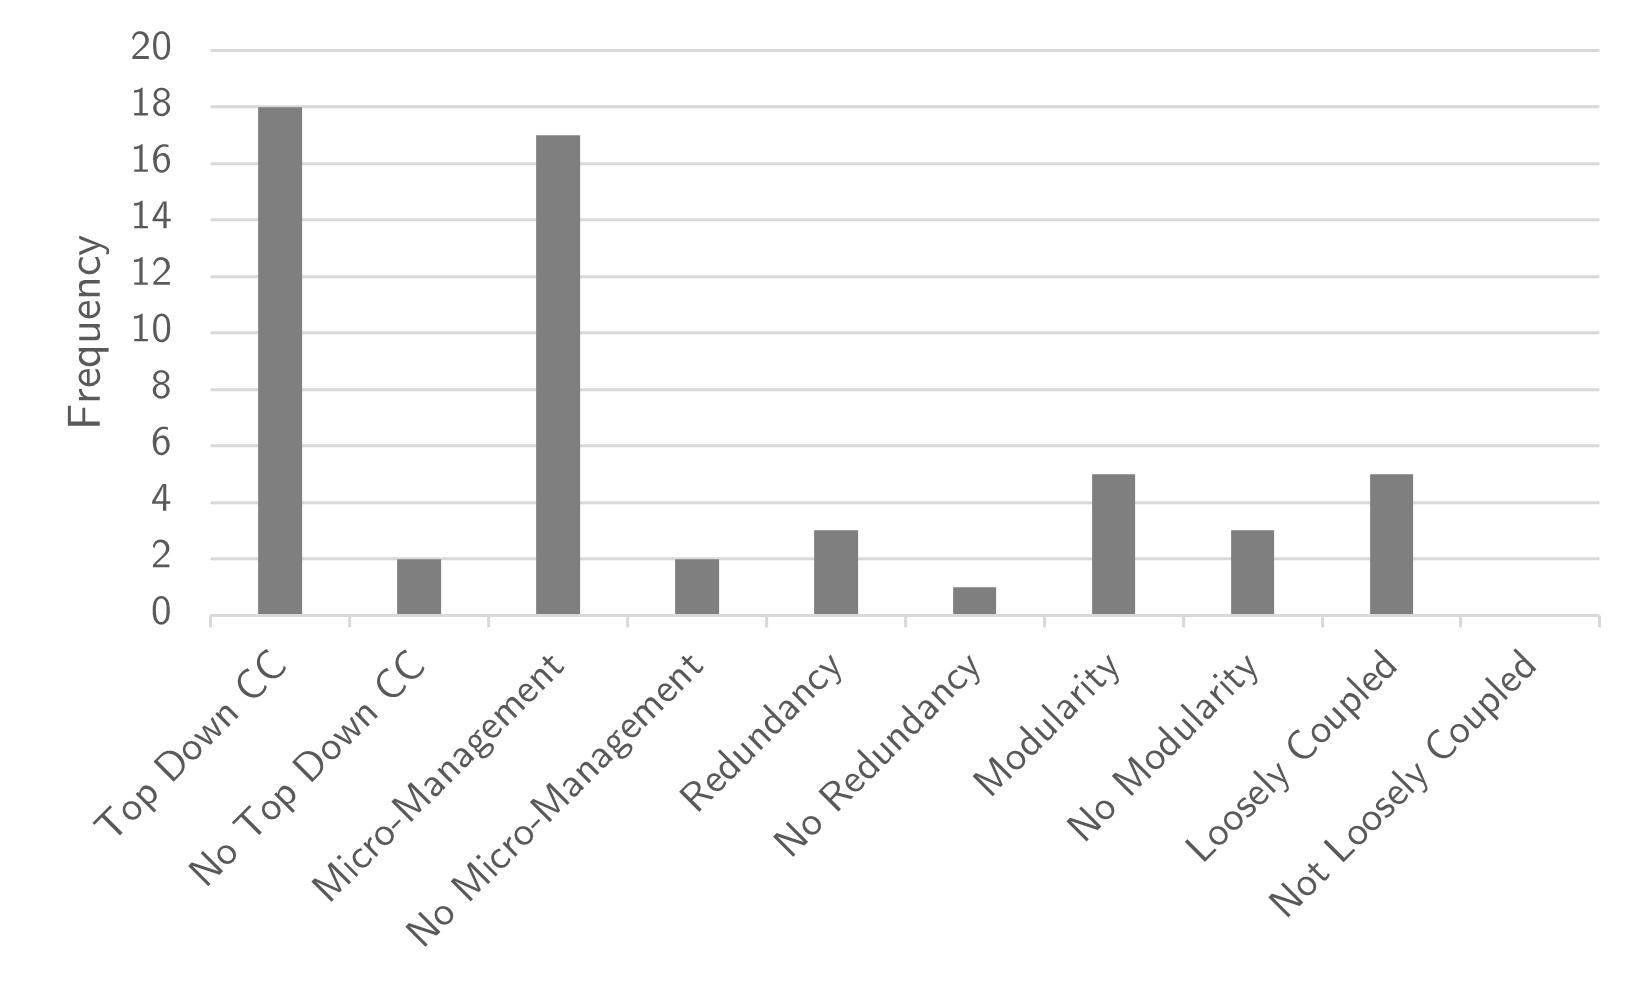
\includegraphics[width=0.95\linewidth]{images/attenuate_frequency}
		\caption[Attenuate variety frequency]{Attenuate variety frequency}
		\label{fig:attenuatefrequency}
	\end{subfigure}%
	\begin{subfigure}[H]{0.5\textwidth}
		\centering
		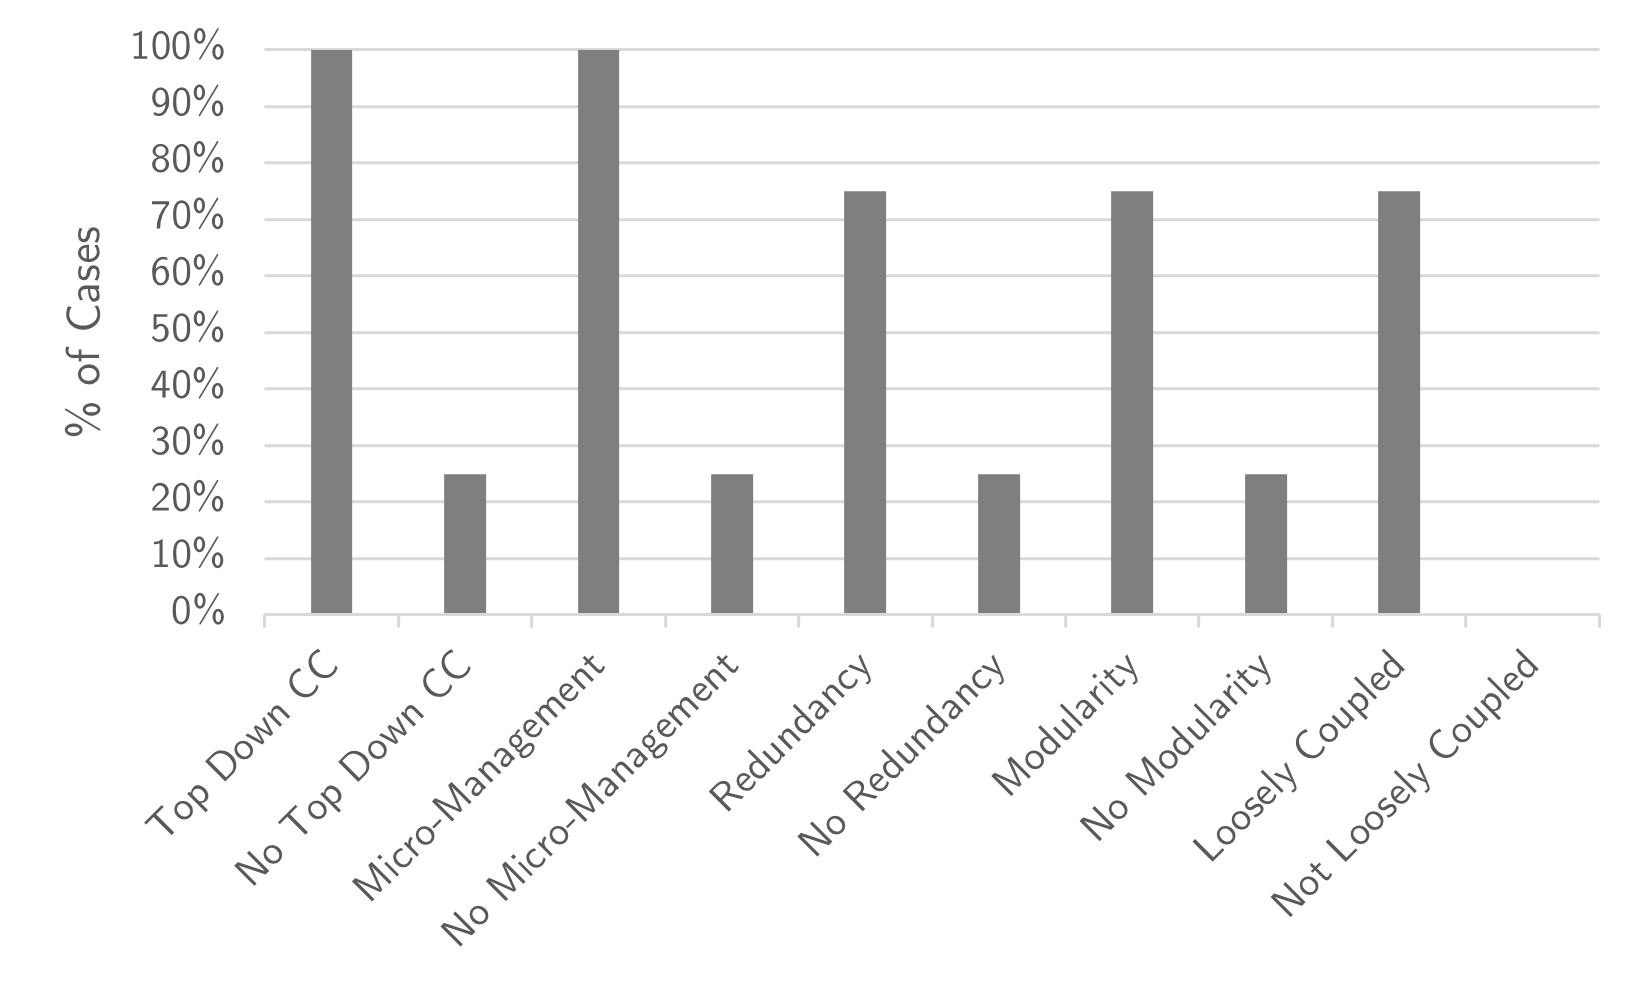
\includegraphics[width=0.95\linewidth]{images/attenuate_cases}
		\caption[Attenuate variety \% of cases]{Attenuate variety \% of cases}
		\label{fig:attenuatecases}
	\end{subfigure}
	\caption[Interview results attenuate variety]{Interview results attenuate variety}
	\label{fig:interviewattenuatevariety}
\end{figure}
E.g. a missing law with the introduction of electric steps (\cref{sec:interviewlocalgovernment}). It is not a bike, not a motorcycle or a car. The electric step did not fit into the current laws and regulations. The result was that the policy-makers did not approve and tolerated it until law-making was finished. Both \textit{\gls{modularity}} and \textit{\gls{looselycoupled}} scored (\Cref{fig:interviewattenuatevariety}) because the \gls{ps} consists of many sub-systems. Every sub-system has a clear goal and a reason to exist. For E.g. local tax offices have the goal of collecting local taxes, while the social services are in charge of paying benefits. Communication between those subsystems is going through standardised interfaces and is predictable. Although \gls{redundancy} is almost non-existent. Every sub-system has its particular goal and reason to exist and cannot take on public tasks another sub-system is performing (\cref{sec:interviewlocalgovernment}).
\subsection{Interview results on amplify variety}
\label{sub:interviewresultsamplify}
The \gls{attribute} of \gls{amplifyvariety} that scored the highest was the \gls{attribute} \textit{\gls{insertlowlevelstress}} (\Cref{fig:interviewamplifiedvariety}). It is not that there is much tinkering going on in the \gls{ps}. Experimentations are (almost) not possible because of public accountability (\cref{sec:interviewlocalgovernment}). However, because of continuous changing laws, policies and regulations, the subsystems of the \gls{ps} are continuously under stress. Nevertheless, the amount of stress differs per layer of the government. Most interviewees stressed that the central government has less stress than the local governments (\cref{sec:interviewlocalgovernment,sec:interviewisv,sec:interviewconsultancyfirm}). This difference makes sense because of the \gls{subsidiarityprinciple} (\cref{sec:tbpublicsector}). The central government performs public tasks when it is impossible at a more local level. The central government is more about policymaking and is a source of stress for the local governments. 

A dimension of stress is the factor of time. Implementing the laws and policies cannot take longer than until the next elections. The standard period of reign is four years before the new elections. The policy-makers want to finish the implementation before replacement. It happens that it is not achievable in the time given. Because of social coherence of public servants, they still try to implement a law or policy within the given time, but they often fail (\cref{sec:interviewlocalgovernment,sec:interviewisv}).

What stands out is that the \glspl{attribute} \textit{no \gls{nonmonotonicity}} and \textit{no \gls{failfast}} are often mentioned. Both have something to do with each other. \textit{\Gls{failfast}} is about experimentations and working in an \gls{agile} way. Experimentations are almost non-existing because of public accountability. Working in an \gls{agile} way is hard for the \gls{ps}. The end state is not always clear enough with the \gls{agile} way of working, which is in conflict with public responsibility and the importance of the attributes \textit{\gls{topdowncc}} and \textit{\gls{micromanagement}} for the \gls{ps}. With an \gls{agile} way of working, the attribute \textit{\gls{selforganisation}} must be present. The \textit{\gls{selforganisation}} was not mentioned that often in the interviews (\cref{fig:interviewamplifiedvariety}. In this case the \gls{attribute} \textit{\gls{selforganisation}} conflicts with \textit{\gls{topdowncc}} and \textit{\gls{micromanagement}}. The \gls{ps} has a very low risk appetite. Everything must be known and explained in advance (\cref{sec:interviewcentralgovernment,sec:interviewlocalgovernment,sec:interviewisv,sec:interviewconsultancyfirm}). 
\begin{figure}[H]
	\centering
	\begin{subfigure}[H]{0.5\textwidth}
		\centering
		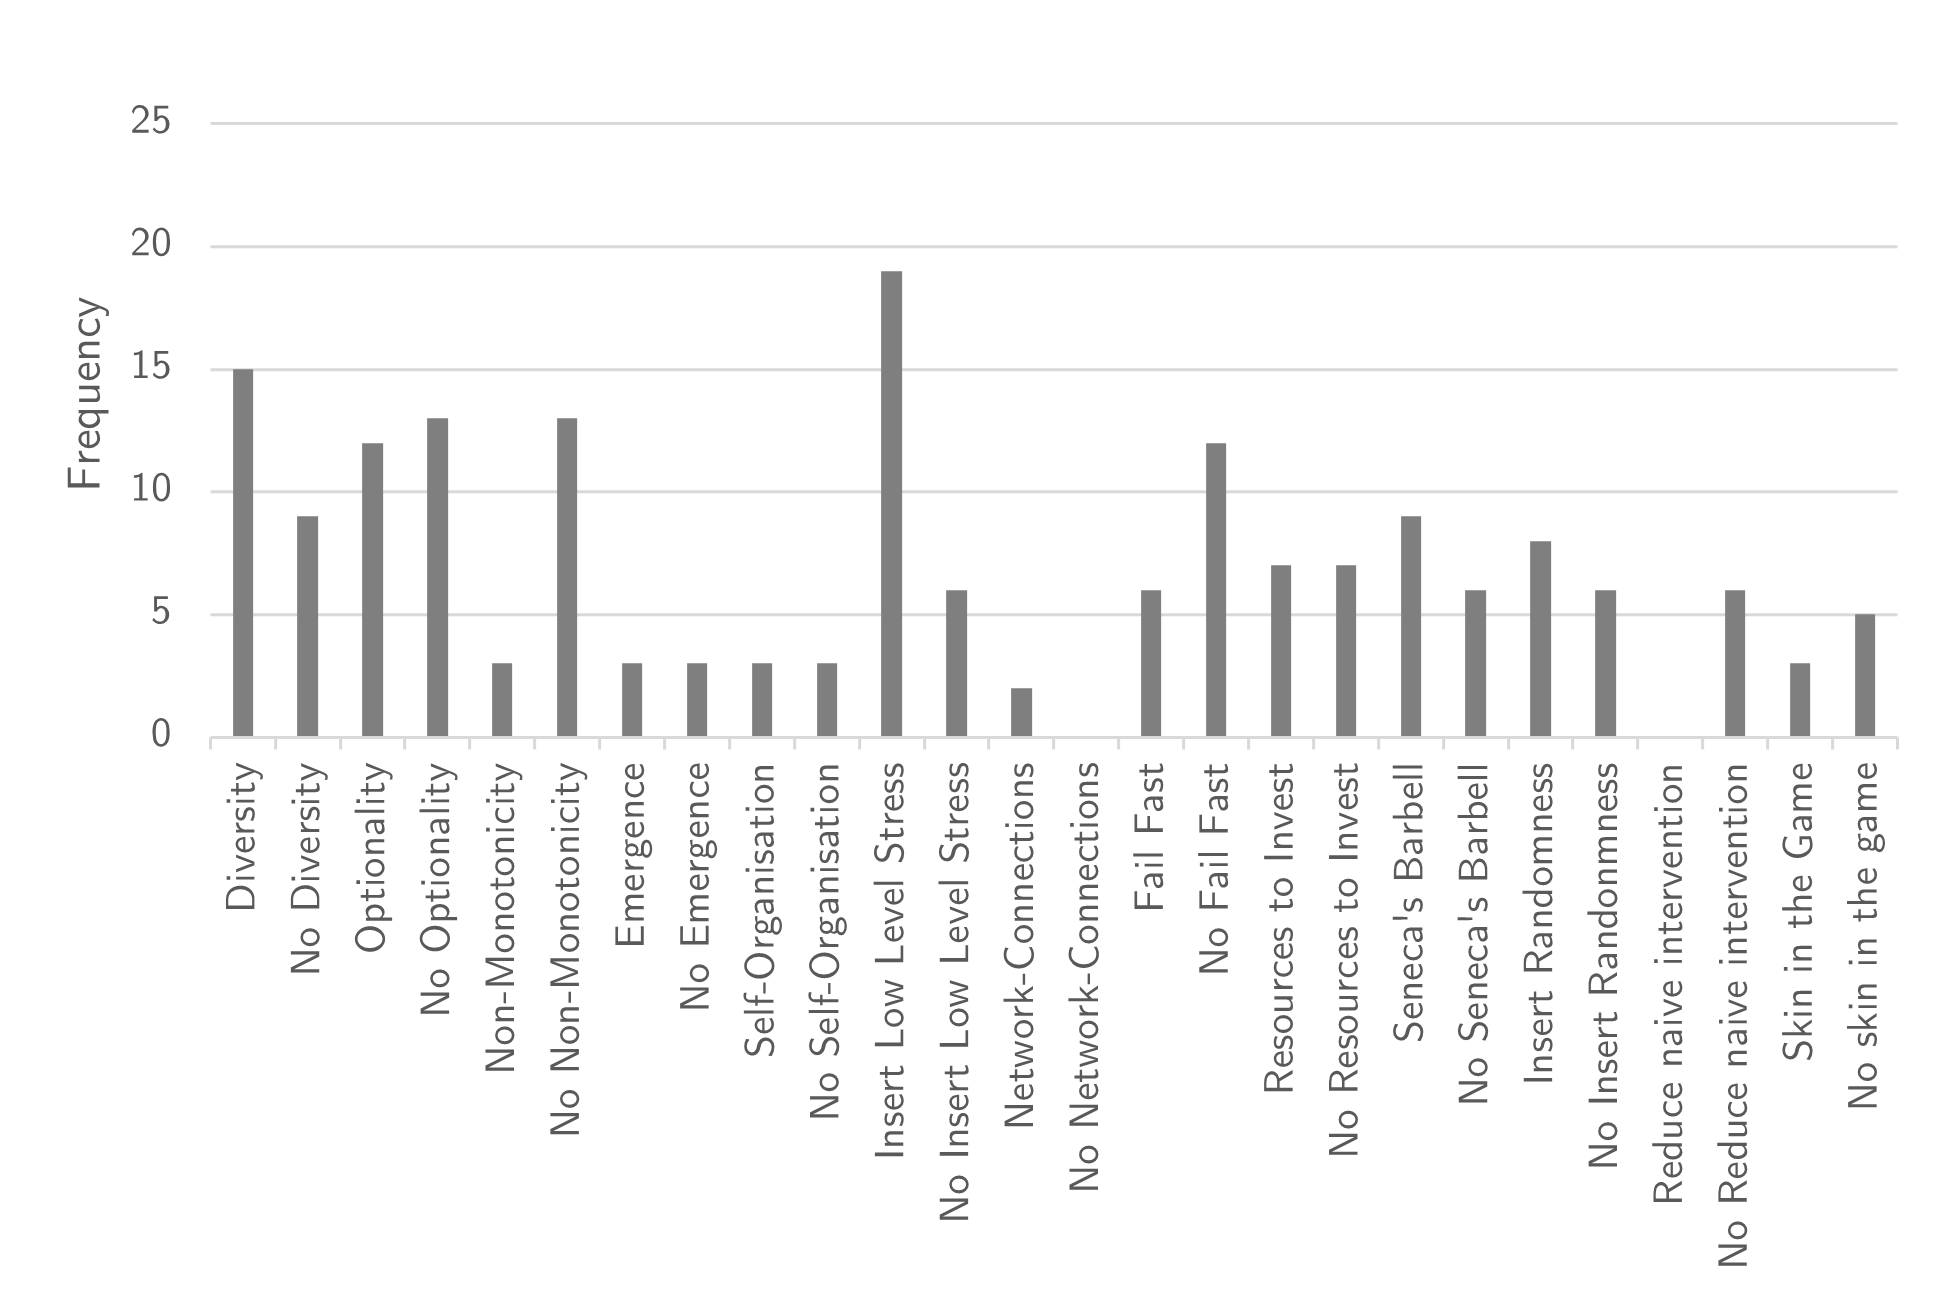
\includegraphics[width=0.95\linewidth]{images/amplified_frequency}
		\caption[Amplified variety frequency]{Amplified variety frequency}
		\label{fig:amplifiedfrequency}
	\end{subfigure}%
	\begin{subfigure}[H]{0.5\textwidth}
		\centering
		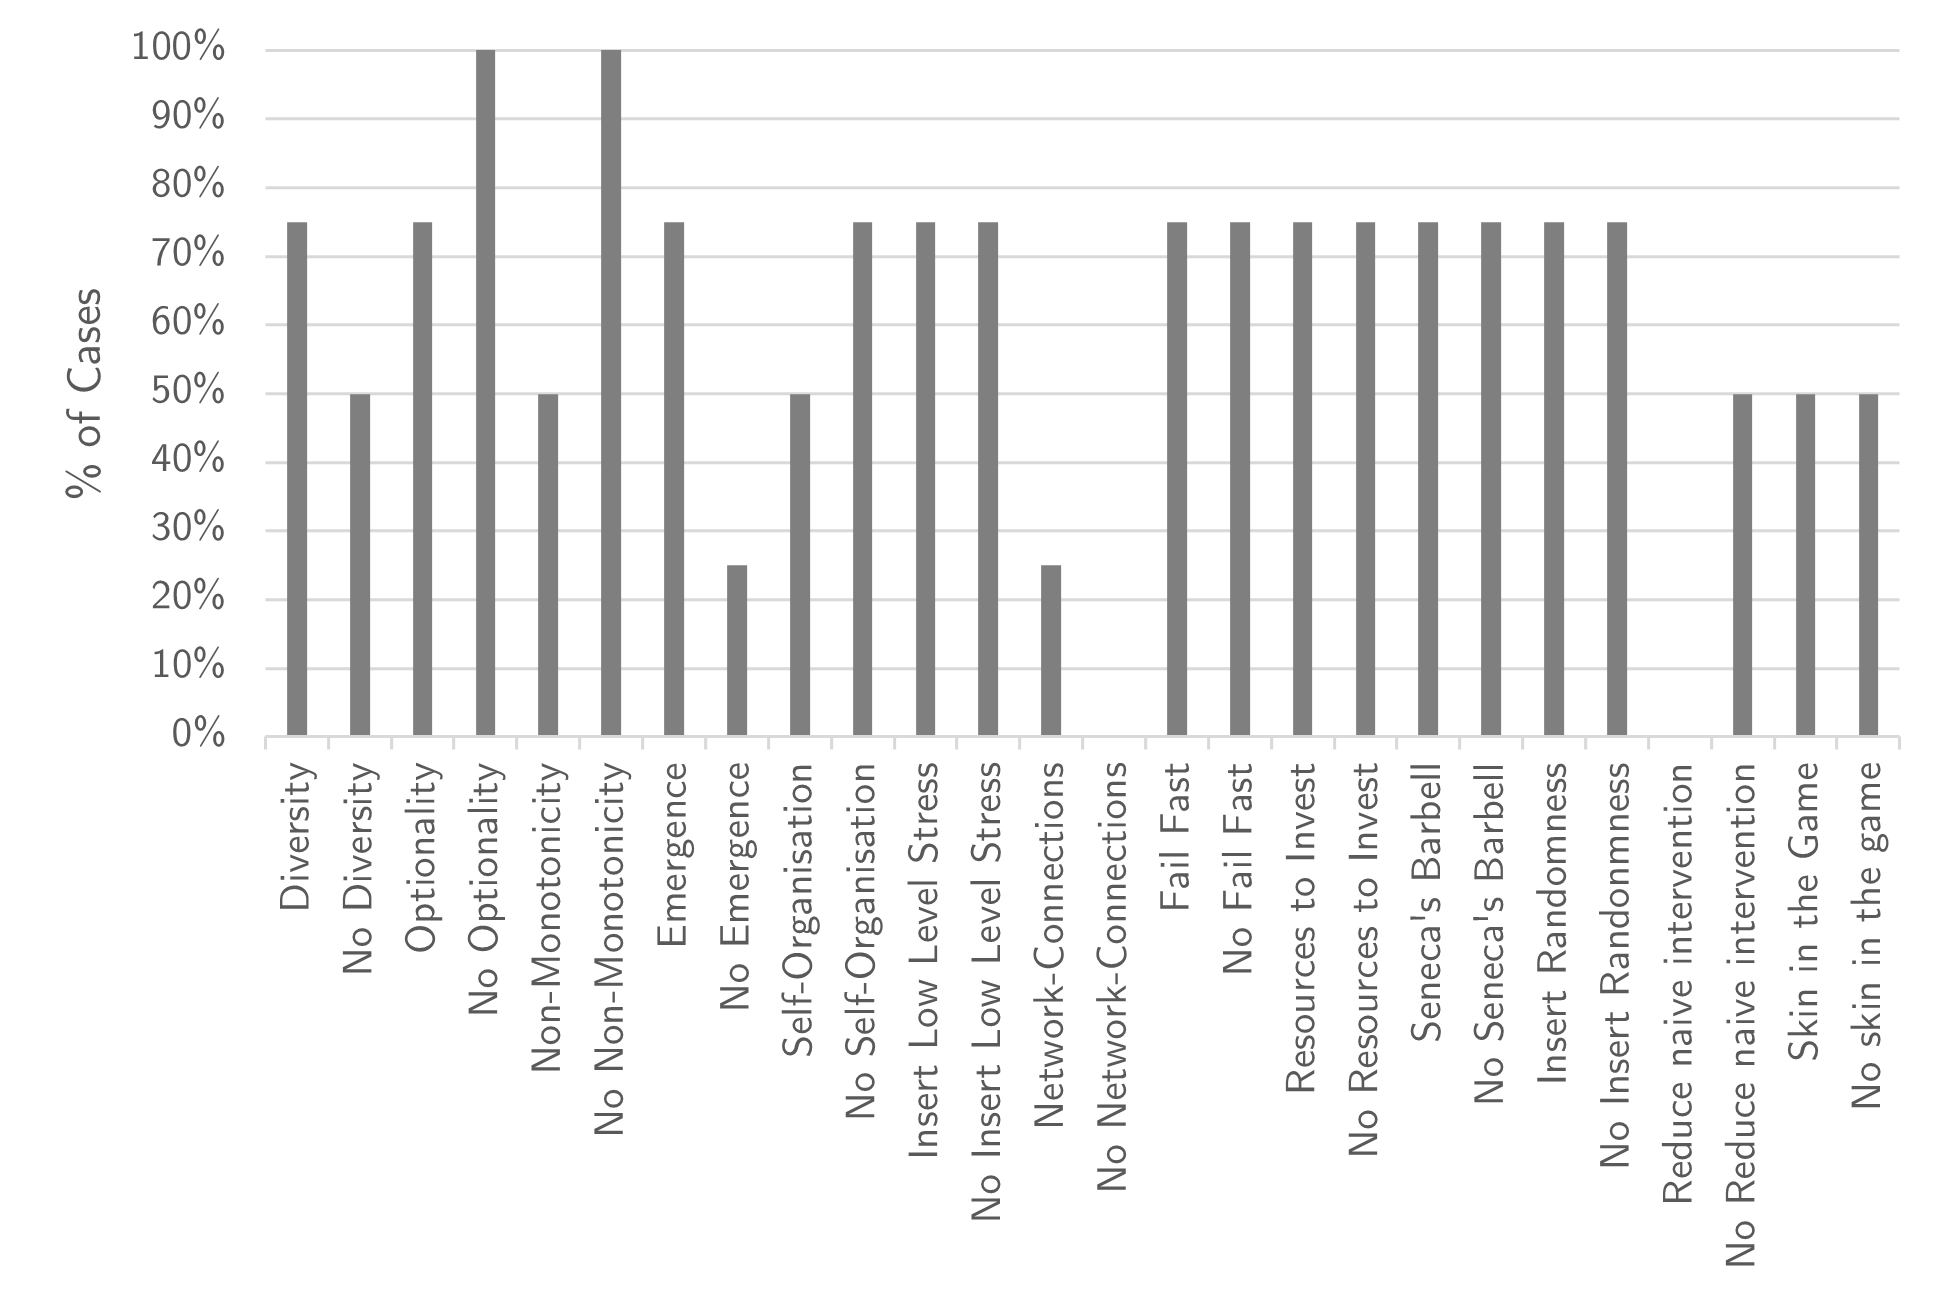
\includegraphics[width=0.95\linewidth]{images/amplified_cases}
		\caption[Amplified variety \% of cases]{Amplified variety \% of cases}
		\label{fig:amplifiedcases}
	\end{subfigure}
	\caption[Interview results amplified variety]{Interview results amplified variety}
	\label{fig:interviewamplifiedvariety}
\end{figure}
\textit{\Gls{nonmonotonicity}} is about learning from previous negative and positive experiences. The \gls{attribute} \textit{\gls{nonmonotonicity}} is not a common practice in the \gls{ps} (\cref{sec:interviewcentralgovernment,sec:interviewisv}). One interviewee even deliberately ignored questions about feedback loops, learning and improving.

\textit{No \gls{optionality}} scored high in frequency, and all the interviewees talked about this in the interviews. The private sector is applying optionality more often. An example given was that of Shell\footnote{https://www.shell.com/} (\cref{sec:interviewisv}). Shell has multiple suppliers for the same product or service. It gives Shell the option to choose between suppliers at any moment in time. Having multiple suppliers for the same product or service are not possible with the \gls{ps}. The \gls{ps} is obliged to comply with public procurement laws. The tender process is mandatory (\cref{sec:interviewcentralgovernment,sec:interviewlocalgovernment,sec:interviewisv,sec:interviewconsultancyfirm}) \parencites{Rijksoverheidaanbesteding}{WTO}.
\subsection{Interview results on learning organisation}
\label{sub:interviewresultslearning}
All interviewees mentioned that when a crisis occurs that they are glad that there are so many artisans working in the \gls{ps}. With a crisis, everyone works toward solutions and acts without conflict of interest. After the crisis is over, everyone falls back into previous behaviour (\cref{sec:interviewlocalgovernment,sec:interviewisv,sec:interviewconsultancyfirm}). Many \glspl{attribute} of a learning organisation are in place in the \gls{ps}. The \glspl{attribute} related to this behaviour are \textit{\gls{personalmastery}}, \textit{\glspl{sharedmentalmodel}}, and \textit{\gls{buildingsharedvision}}. \Cref{fig:interviewlearningorganisation} shows the same.

On the other hand \textit{\gls{systemsthinking}} is less common in the \gls{ps}. Every subsystem has its particular goal and reason to exist and cannot perform public tasks another subsystem is responsible for (\cref{sub:interviewresultsattenuate}). The \gls{ps} does not foster thinking outside of a sub-system.
\begin{figure}[H]
	\centering
	\begin{subfigure}[H]{0.5\textwidth}
		\centering
		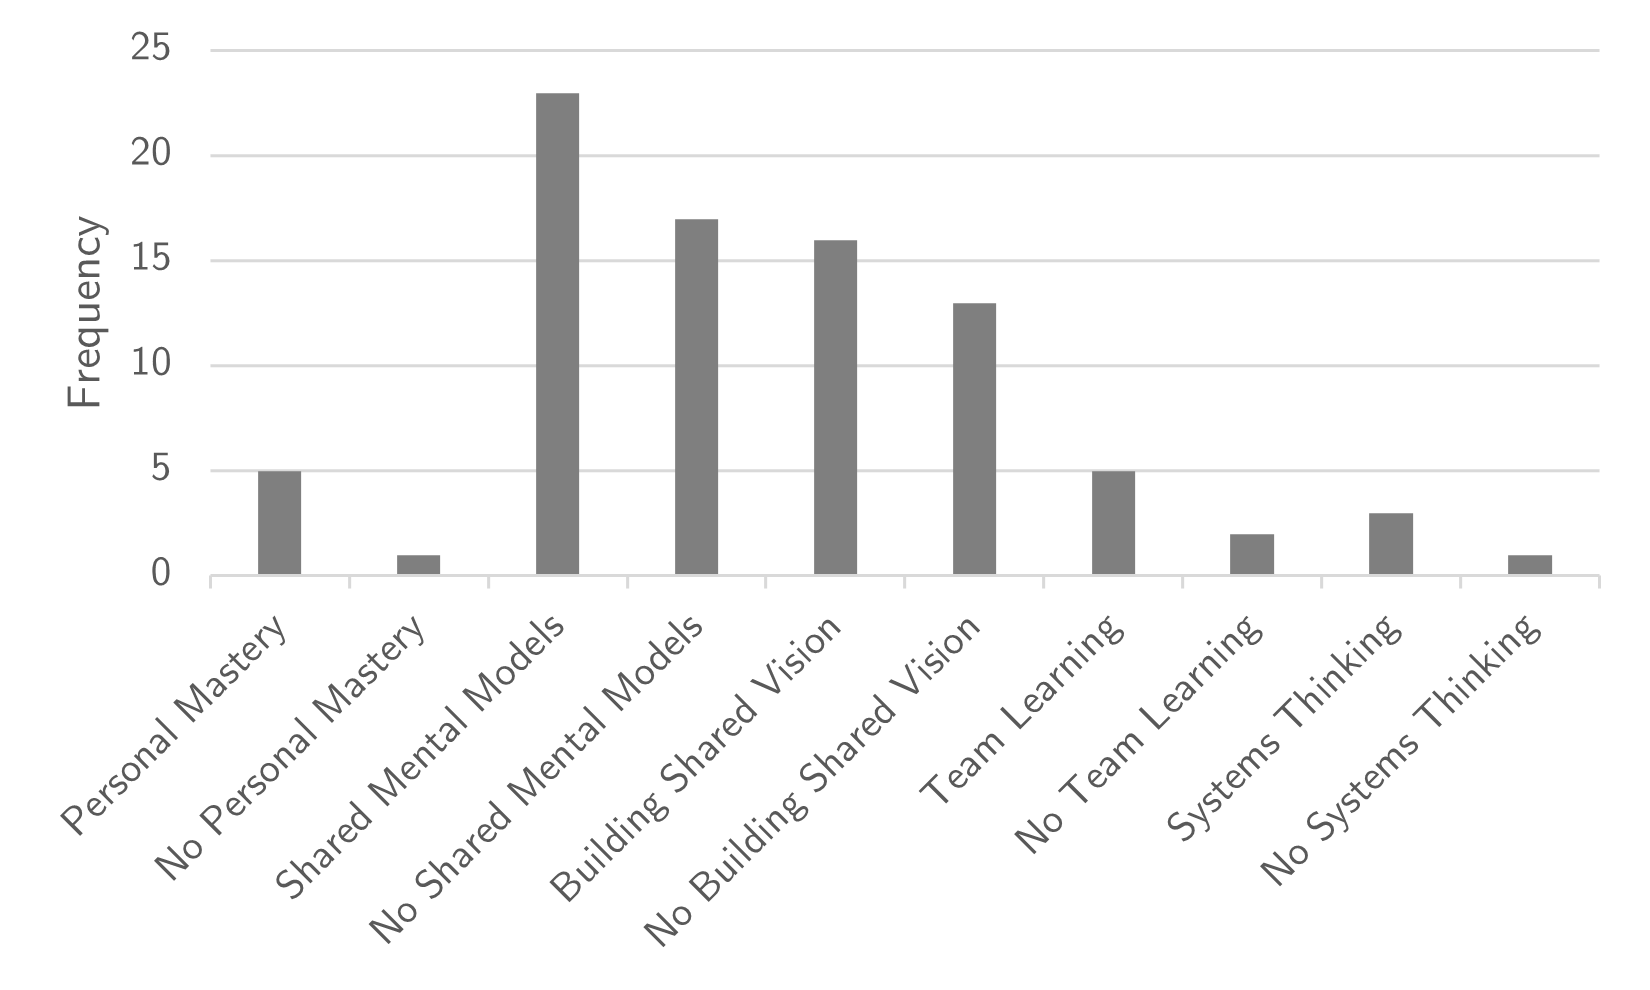
\includegraphics[width=0.95\linewidth]{images/learningorganisation_frequency}
		\caption{Learning organisation frequency}
		\label{fig:learningfrequency}
	\end{subfigure}%
	\begin{subfigure}[H]{0.5\textwidth}
		\centering
		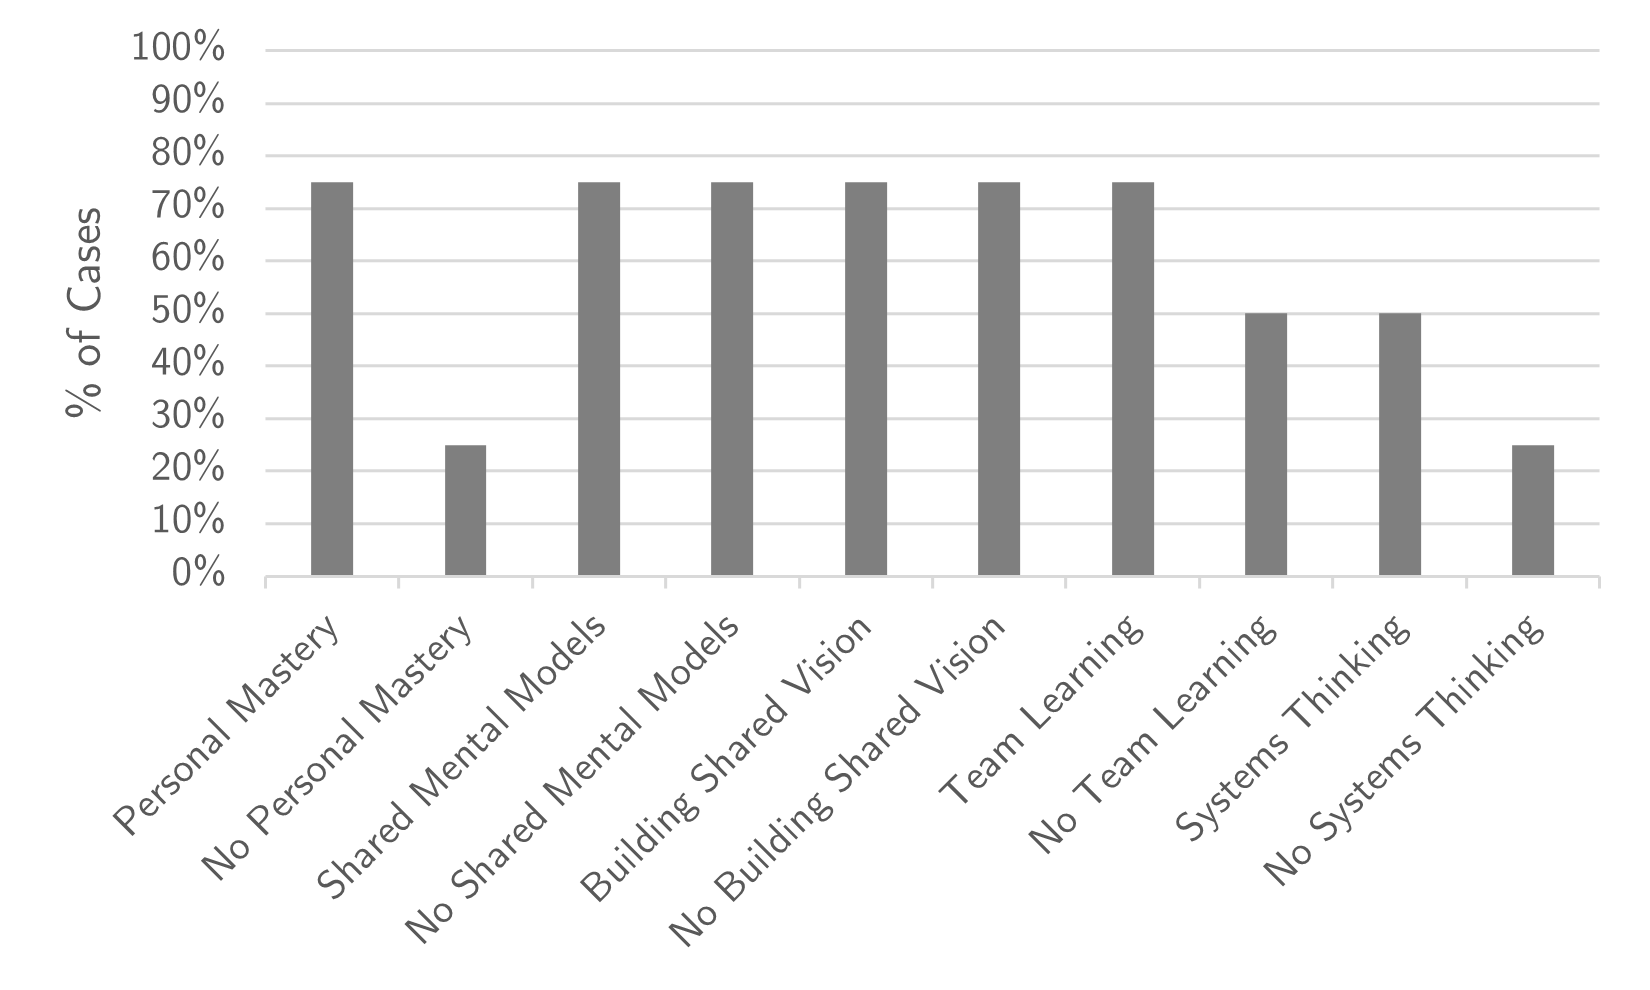
\includegraphics[width=0.95\linewidth]{images/learningorganisation_cases}
		\caption{Learning organisation \% of cases}
		\label{fig:learningcases}
	\end{subfigure}
	\caption{Interview results learning organisation}
	\label{fig:interviewlearningorganisation}
\end{figure}

\subsection{Interview results on Enterprise Architecture schools of thought}
\label{sub:interviewresultseaschools}
The concern for this category was what the most common \acrlong{ea} school of thought (\cref{sub:eaapproaches}) is in the Dutch \gls{ps}. Al three schools of thought were present in the interviews. Nevertheless, the school of thought \textit{\gls{enterpriseitarchitecting}} was present in three interviews (\cref{fig:intervieweaschoolsantifragile}). In contrast, the schools \textit{\gls{enterpriseintegrating}} and \textit{\gls{enterpriseecologicaladaptation}} were present in two, but different, interviews.
\begin{figure}[H]
	\centering
	\begin{subfigure}[H]{0.5\textwidth}
		\centering
		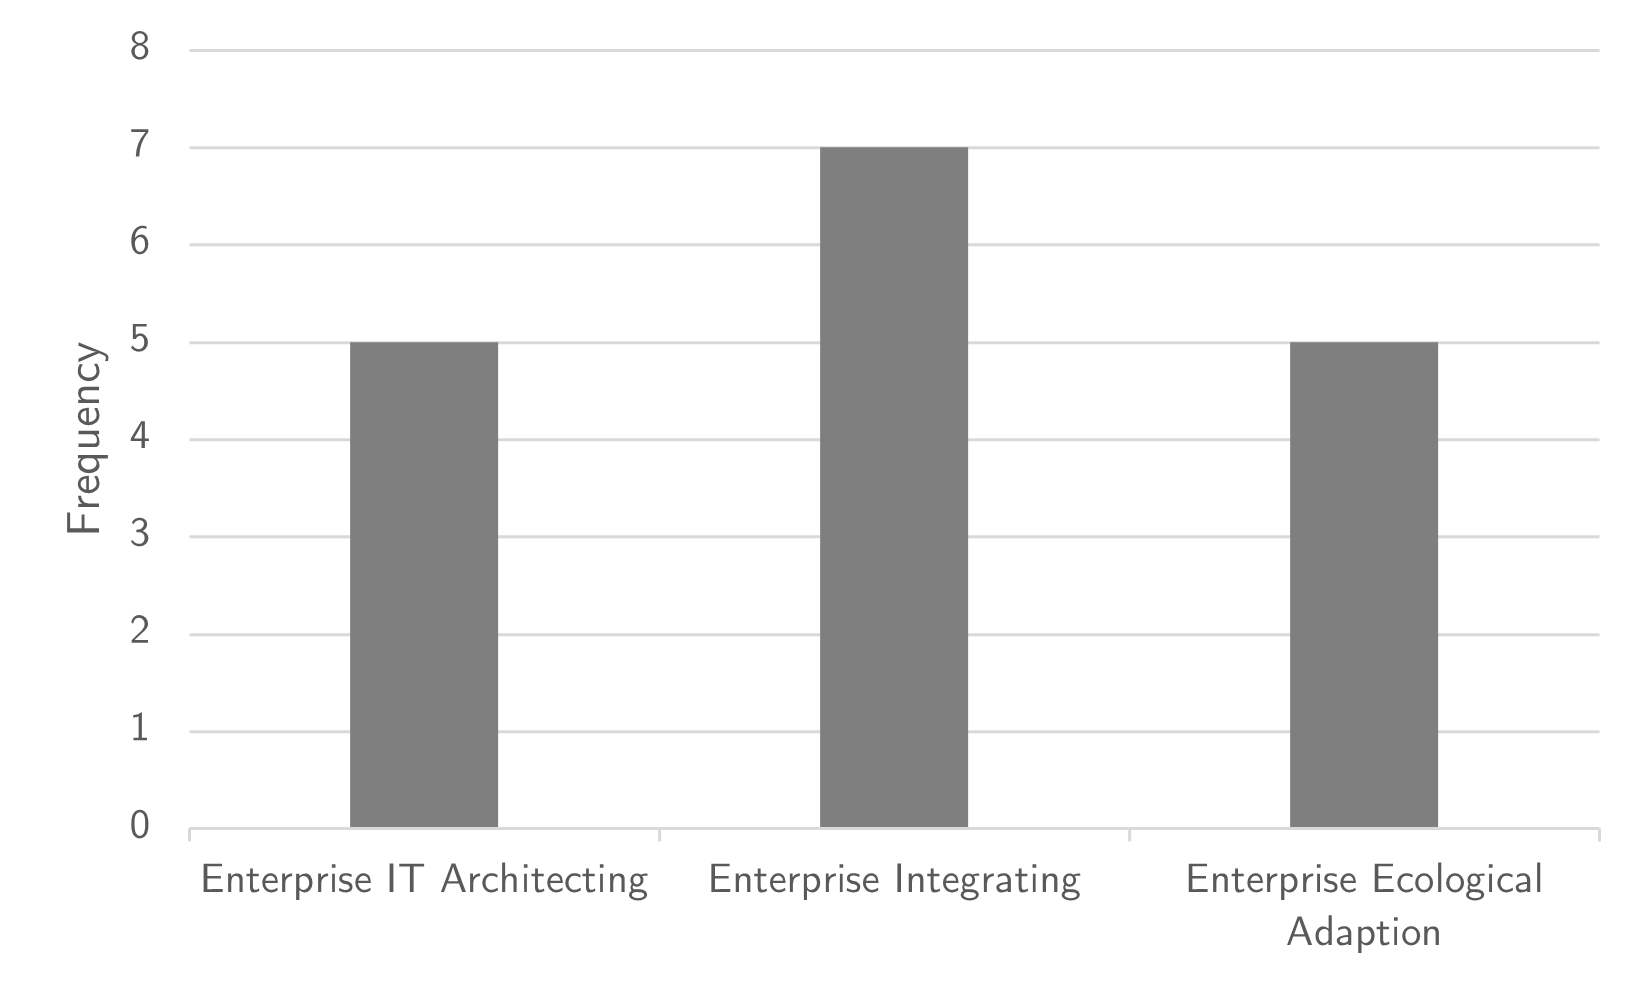
\includegraphics[width=0.95\linewidth]{images/easchools_frequency}
		\caption{Enterprise Architecture Schools of thought Frequency}
		\label{fig:easchoolsfrequency}
	\end{subfigure}%
	\begin{subfigure}[H]{0.5\textwidth}
		\centering
		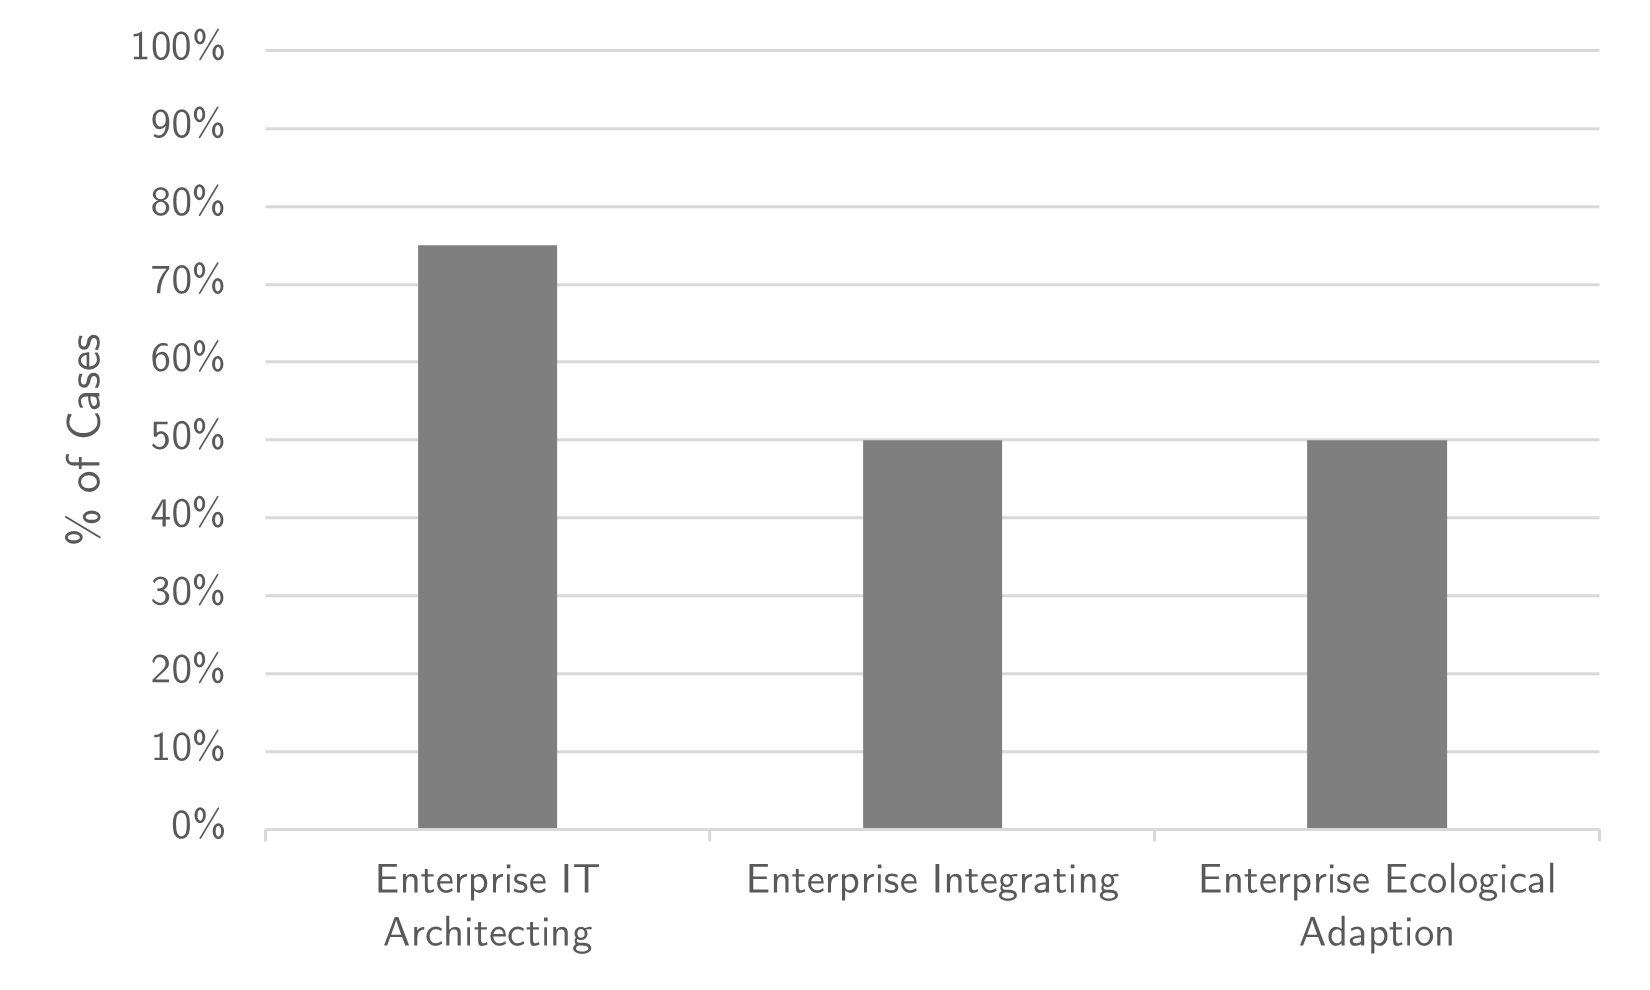
\includegraphics[width=0.95\linewidth]{images/easchools_cases}
		\caption{Enterprise Architecture Schools of thought \% of Cases}
		\label{fig:easchoolscases}
	\end{subfigure}
	\caption{Interview results Enterprise Architecture schools of thought}
	\label{fig:intervieweaschoolsantifragile}
\end{figure}
There are differences in the practice of \acrshort{ea} between the organisations of the interviewees. Two of the interviewees are practising \acrshort{ea} mainly in the school of thought \textit{\gls{enterpriseitarchitecting}} (\cref{sec:interviewcentralgovernment,sec:interviewlocalgovernment}). One of the interviewees is in the school of thought \textit{\gls{enterpriseitarchitecting}} but has already started to show signs of \textit{\gls{enterpriseintegrating}} (\cref{sec:interviewconsultancyfirm}). They are more aware of the environment, and they are starting to use \acrshort{ea} as a means to implement the enterprise strategy of the organisation. The last interviewee operates mainly in the school of thought \textit{\gls{enterpriseintegrating}} and is moving more to \textit{\gls{enterpriseecologicaladaptation}} (\cref{sec:interviewisv}). The organisation of the interviewee is not only using \acrshort{ea} to manage the environment, but they are starting to use \acrshort{ea} to change the environment. They do this by actively participating in decision-making and policy-making in the \gls{ps}. However, most of the interviewees agree that practising \acrshort{ea} in the \gls{ps} as a \acrlong{sos} is likely the \acrshort{ea} school of thought of \textit{\gls{enterpriseitarchitecting}}.

With the interviews, it became clear that the \gls{ps} is not using \acrshort{ea} as an instrument for decision-making (\cref{sec:interviewcentralgovernment,sec:interviewlocalgovernment,sec:interviewisv}). \acrshort{ea} follows after decision-making in the sub-systems. The result is that \acrshort{ea} is always running behind on the policies, laws and decisions. Accordingly to the interviewees, this has its origin in that the policy-makers and decision-makers do not understand \acrshort{ea}. One interviewee gave the example of the land surveyor\footnote{\url{https://en.wikipedia.org/wiki/Surveying}} profession (\cref{sec:interviewlocalgovernment}). The land surveyor learns to speak the language of its stakeholders. By using the stakeholder's natural language to communicate measurements and concerns, the stakeholders understand the meaning. All interviewees have the opinion that \acrshort{ea} does not communicate in the stakeholder's natural language. As long as \acrshort{ea} does not communicate in the natural language of the stakeholder, \acrshort{ea} will not be involved in decision-making and policy-making. This finding resulted in a possible new \gls{attribute} regarding success factors. This new \gls{attribute} is noted in \cref{fig:interviewresultsfindings}.
\subsection{Interview results on possible new attributes}
\label{sub:interviewresultsnewattributes}
The last category of \glspl{attribute} for discussion is the category of new findings. The newly found \glspl{attribute} \mbox{(\cref{fig:interviewresultsfindings})} were discovered conducting interviews. Most of the findings are already discussed in the previous sub-sections. These are findings like \textit{adapt to business language}, \textit{limited \acrshort{ea}}, \textit{governance}, \textit{public responsibility} and \textit{risk avoidance}. 
\begin{figure}[H]
	\centering
	\begin{subfigure}[H]{0.5\textwidth}
		\centering
		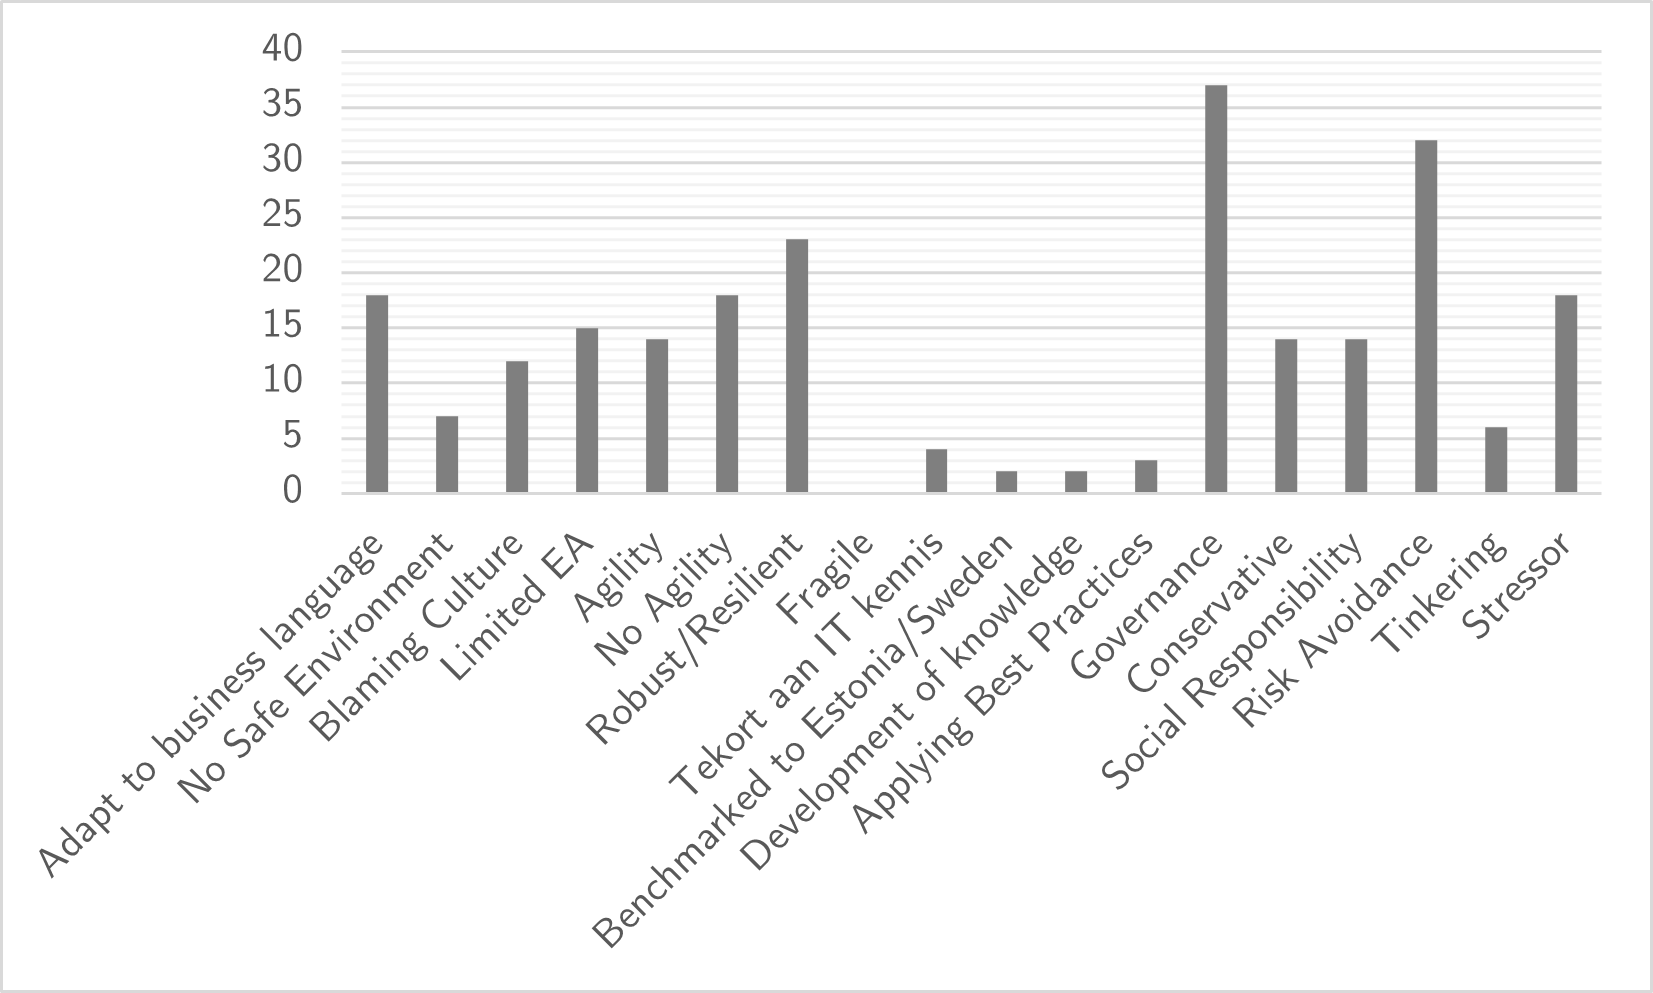
\includegraphics[width=0.95\linewidth]{images/findings_frequency}
		\caption{New findings frequency}
		\label{fig:findingsfrequency}
	\end{subfigure}%
	\begin{subfigure}[H]{0.5\textwidth}
		\centering
		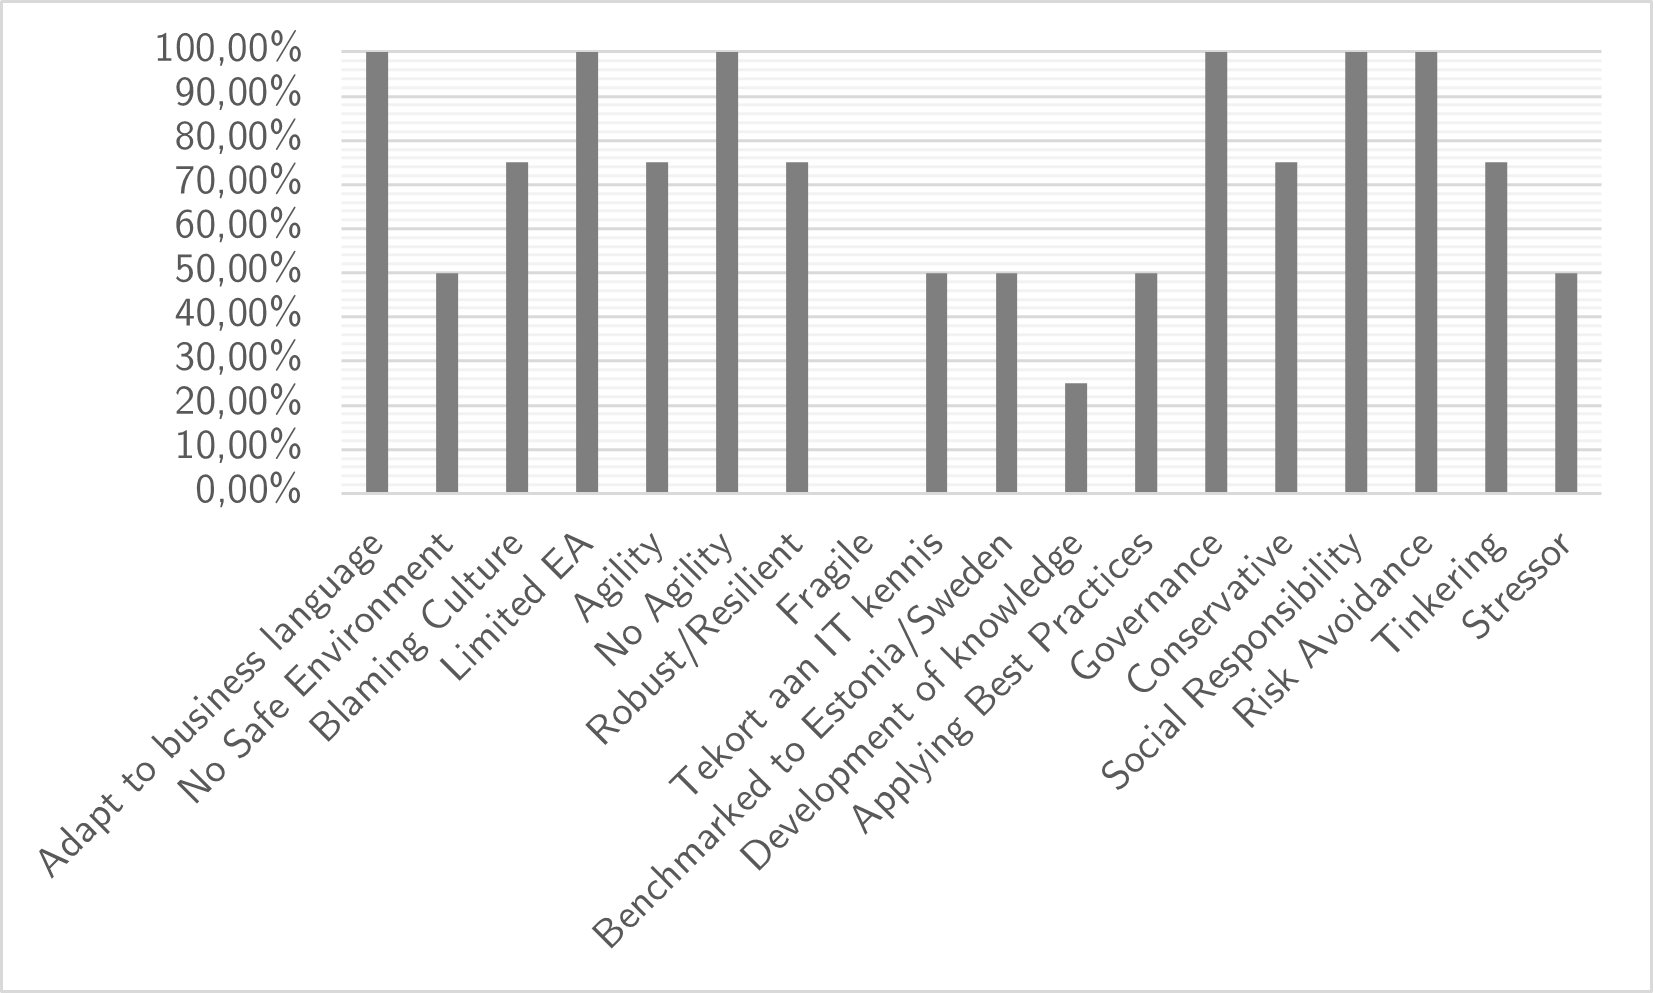
\includegraphics[width=0.95\linewidth]{images/findings_cases}
		\caption{New findings \% of cases}
		\label{fig:findingscases}
	\end{subfigure}
	\caption{Interview results new findings}
	\label{fig:interviewresultsfindings}
\end{figure}
Of the new findings that are not yet treated, the most important two are \textit{blaming culture} and \textit{no \gls{safeworkingenvironment}}. The two were mentioned often across all the topics. The two are related. \textit{No \gls{safeworkingenvironment}} can be the result of a \textit{blaming culture}. All the interviews talked about how in a crisis, people do anything to solve it. However, since the \gls{ps} is all about public accountability, all processes need to be followed. Everything must be predefined and planned (\cref{sub:interviewresultsattenuate}). Most of the time, the processes are slowing it down, while it should go faster in a crisis. After the crisis, there are possible \glspl{parliamentaryinquiry}, and there is \acrshort{bit} who is responsible for overseeing and auditing all \acrshort{it} projects of the central governments. Both are not accepting deviations in processes. Even with a successful result, there is a possibility of severe consequences. This is what we call a \textit{blaming culture}. The result of this behaviour in the \gls{ps} is that people are not willing to take risks. They are afraid of possible repercussions. There is not a \gls{safeworkingenvironment} in the \gls{ps} for people to self-organise or to excel. However, it is not this black and white. It is less with the regional and local governments. It is the strongest with the central governments (\cref{sec:interviewlocalgovernment,sec:interviewisv}).
\section{Qualitative Data Analysis}
\label{sec:dataprep}
Until now, we have interview results with an explanation of attribute presence in the \gls{ps}. However, with these results, we still cannot say which attributes are of any significance for \gls{antifragile} and \acrshort{ea} in the \gls{ps}. As already stated earlier in \cref{sec:interviewresults}, we need \acrshort{qda} for data interpretation. The data set used for the \acrshort{qda} is available as a structured Microsoft Excel workbook with multiple worksheets. This file is available in the GitHub repository of this research\footnote{\url{https://github.com/JRBliekendaal/master-thesis/blob/57f1489c59832d4c94d8bd6726d4e260f8ad544e/datasets/interviews/qda_steps.xlsx}}. The first step in the \acrshort{qda} is analysing and merging labels (\cref{tab:prepmergingsimilarlabels}). Positive and negative labels were created for the main categories for possible overarching findings. Merging findings with already existing \glspl{attribute} was next. The \glspl{attribute} left are new, not an \gls{attribute} but something else, or just a note to remember something. The analysis did not include the last two. 
\begin{longtable}{@{}p{.05\textwidth}p{.4\textwidth}p{.4\textwidth}@{}}
	\toprule%
	\textbf{Step} & \textbf{Description} & \textbf{Rationale} \\%
	\midrule%
	\endhead%
	\hline
	\endfoot%
	\caption[Merging similar labels]{Merging similar labels}
	\label{tab:prepmergingsimilarlabels}
	\endlastfoot%
	1	  & Create, positive and negative main categories of Engineering, Systems, CAS, \gls{antifragile}, and Learning organisation. & Need extra categories for merging overarching subjects. \\%
	2     & Merge \gls{agility} into CAS & How \gls{agility} is interpreted is the same as CAS \\%
	3     & Merge tinkering into Learning Organisation & How tinkering is interpreted it is the same as Learning Organisation. \\%
	4     & Merge \gls{robust} and \gls{resilient} into Engineering Resilience & How \gls{robust} and \gls{resilient} is interpreted by interviewees is the same as Engineering Resilience. \\%
	5     & Merge Governance into Engineering Resilience & How Governance is interpreted is the same as \gls{topdowncc} and \gls{micromanagement}. \\%
	6     & Merge Shortage on IT Knowledge into no \gls{resourcestoinvest} & Shortage on IT Knowledge can be interpreted as a resource that is not there \\%
	7     & Merge Applying Best practices into \gls{nonmonotonicity} & Applying Best practices is learning from the past. \\%
	8     & Merge Development of Knowledge into Learning Organisation & Development of Knowledge within an organisation can be seen as the learning capability of an organisation. \\%
	9     & Merge Blaming Culture into No Safe Environment & No Safe Environment is a result of a Blaming Culture. \\%
	10    & Merge Limited \acrshort{ea} into \gls{enterpriseitarchitecting} & Limited \acrshort{ea} is interpreted as the school of thought \gls{enterpriseitarchitecting} \\%
	11    & Merge conservative into Risk Avoidance & Risk Avoidance is a result of conservative \\%
	12	  & Ignored Public Responsibility and Risk Avoidance as \glspl{attribute} as possible success factors & Public Responsibility and Risk Avoidance are attributes of the \gls{ps} and are less relevant as an attribute for \gls{antifragile} and \acrshort{ea}. \\%
	\bottomrule%
\end{longtable}%
Normalising the frequency of \glspl{attribute} prevented bias of the interviewees. The presence of an attribute was only counted once per question per interview. Twenty-eight was the maximum score with four interviews and seven main questions.
 
Interpretation is still not possible at this moment in the \acrshort{qda}. There are still two \glspl{attribute} for most \glspl{attribute}, one negative and one positive. Subtracting the negative \gls{attribute} from the positive resulted in a score for the primary \gls{attribute}. The result of normalisation is that the \glspl{attribute} are comparable. If the score is positive, the \gls{attribute} is already a property of the \gls{ps} and inversely. A positive \gls{attribute} is not of any significance, but a negative \gls{attribute} could be. A negative attribute is an property that is absent in the \gls{ps}.
 
Before defining the significance of \glspl{attribute}, it is necessary to determine how widely supported an \glspl{attribute} is. An \gls{attribute} only mentioned during one interview is not a widely supported \gls{attribute}. The chance that this is a success factor for the \gls{ps} is low. It is at most a success factor for the sub-system of the interviewee. We decided to use a threshold of three out of four (75\%). When three or more interviews mentioned the attribute, it could be an attribute of any significance.

After performing \acrshort{qda}, the interview findings are interpreted. When there is a score of zero or less for \gls{attenuatevariety}, \gls{amplifyvariety}, and learning organisation \glspl{attribute}, then the \gls{attribute} has some degree of certainty that it has a positive influence on achieving \gls{antifragility} in the \gls{ps}. \Glspl{attribute} that scored 0 or less are \textit{\gls{optionality}}, \textit{\gls{nonmonotonicity}}, \textit{\gls{selforganisation}}, \textit{\gls{failfast}}, \textit{\gls{resourcestoinvest}} and \textit{\gls{senecabarbell}} (\cref{fig:scoreofattributes}). All of these \glspl{attribute} are from the category \gls{amplifyvariety}.

The interpretation of the score of the newly found \glspl{attribute} is different. The interpretation of these \glspl{attribute} is that they must exist. Both the \glspl{attribute} mentioned have some degree of certainty that it has a positive influence on achieving \gls{antifragility} in the \gls{ps}. These attributes are \textit{\gls{adapttobusinesslanguage}} and \textit{\gls{safeworkingenvironment}} (\cref{fig:scoreofattributes}).
\begin{figure}[H]
	\centering
	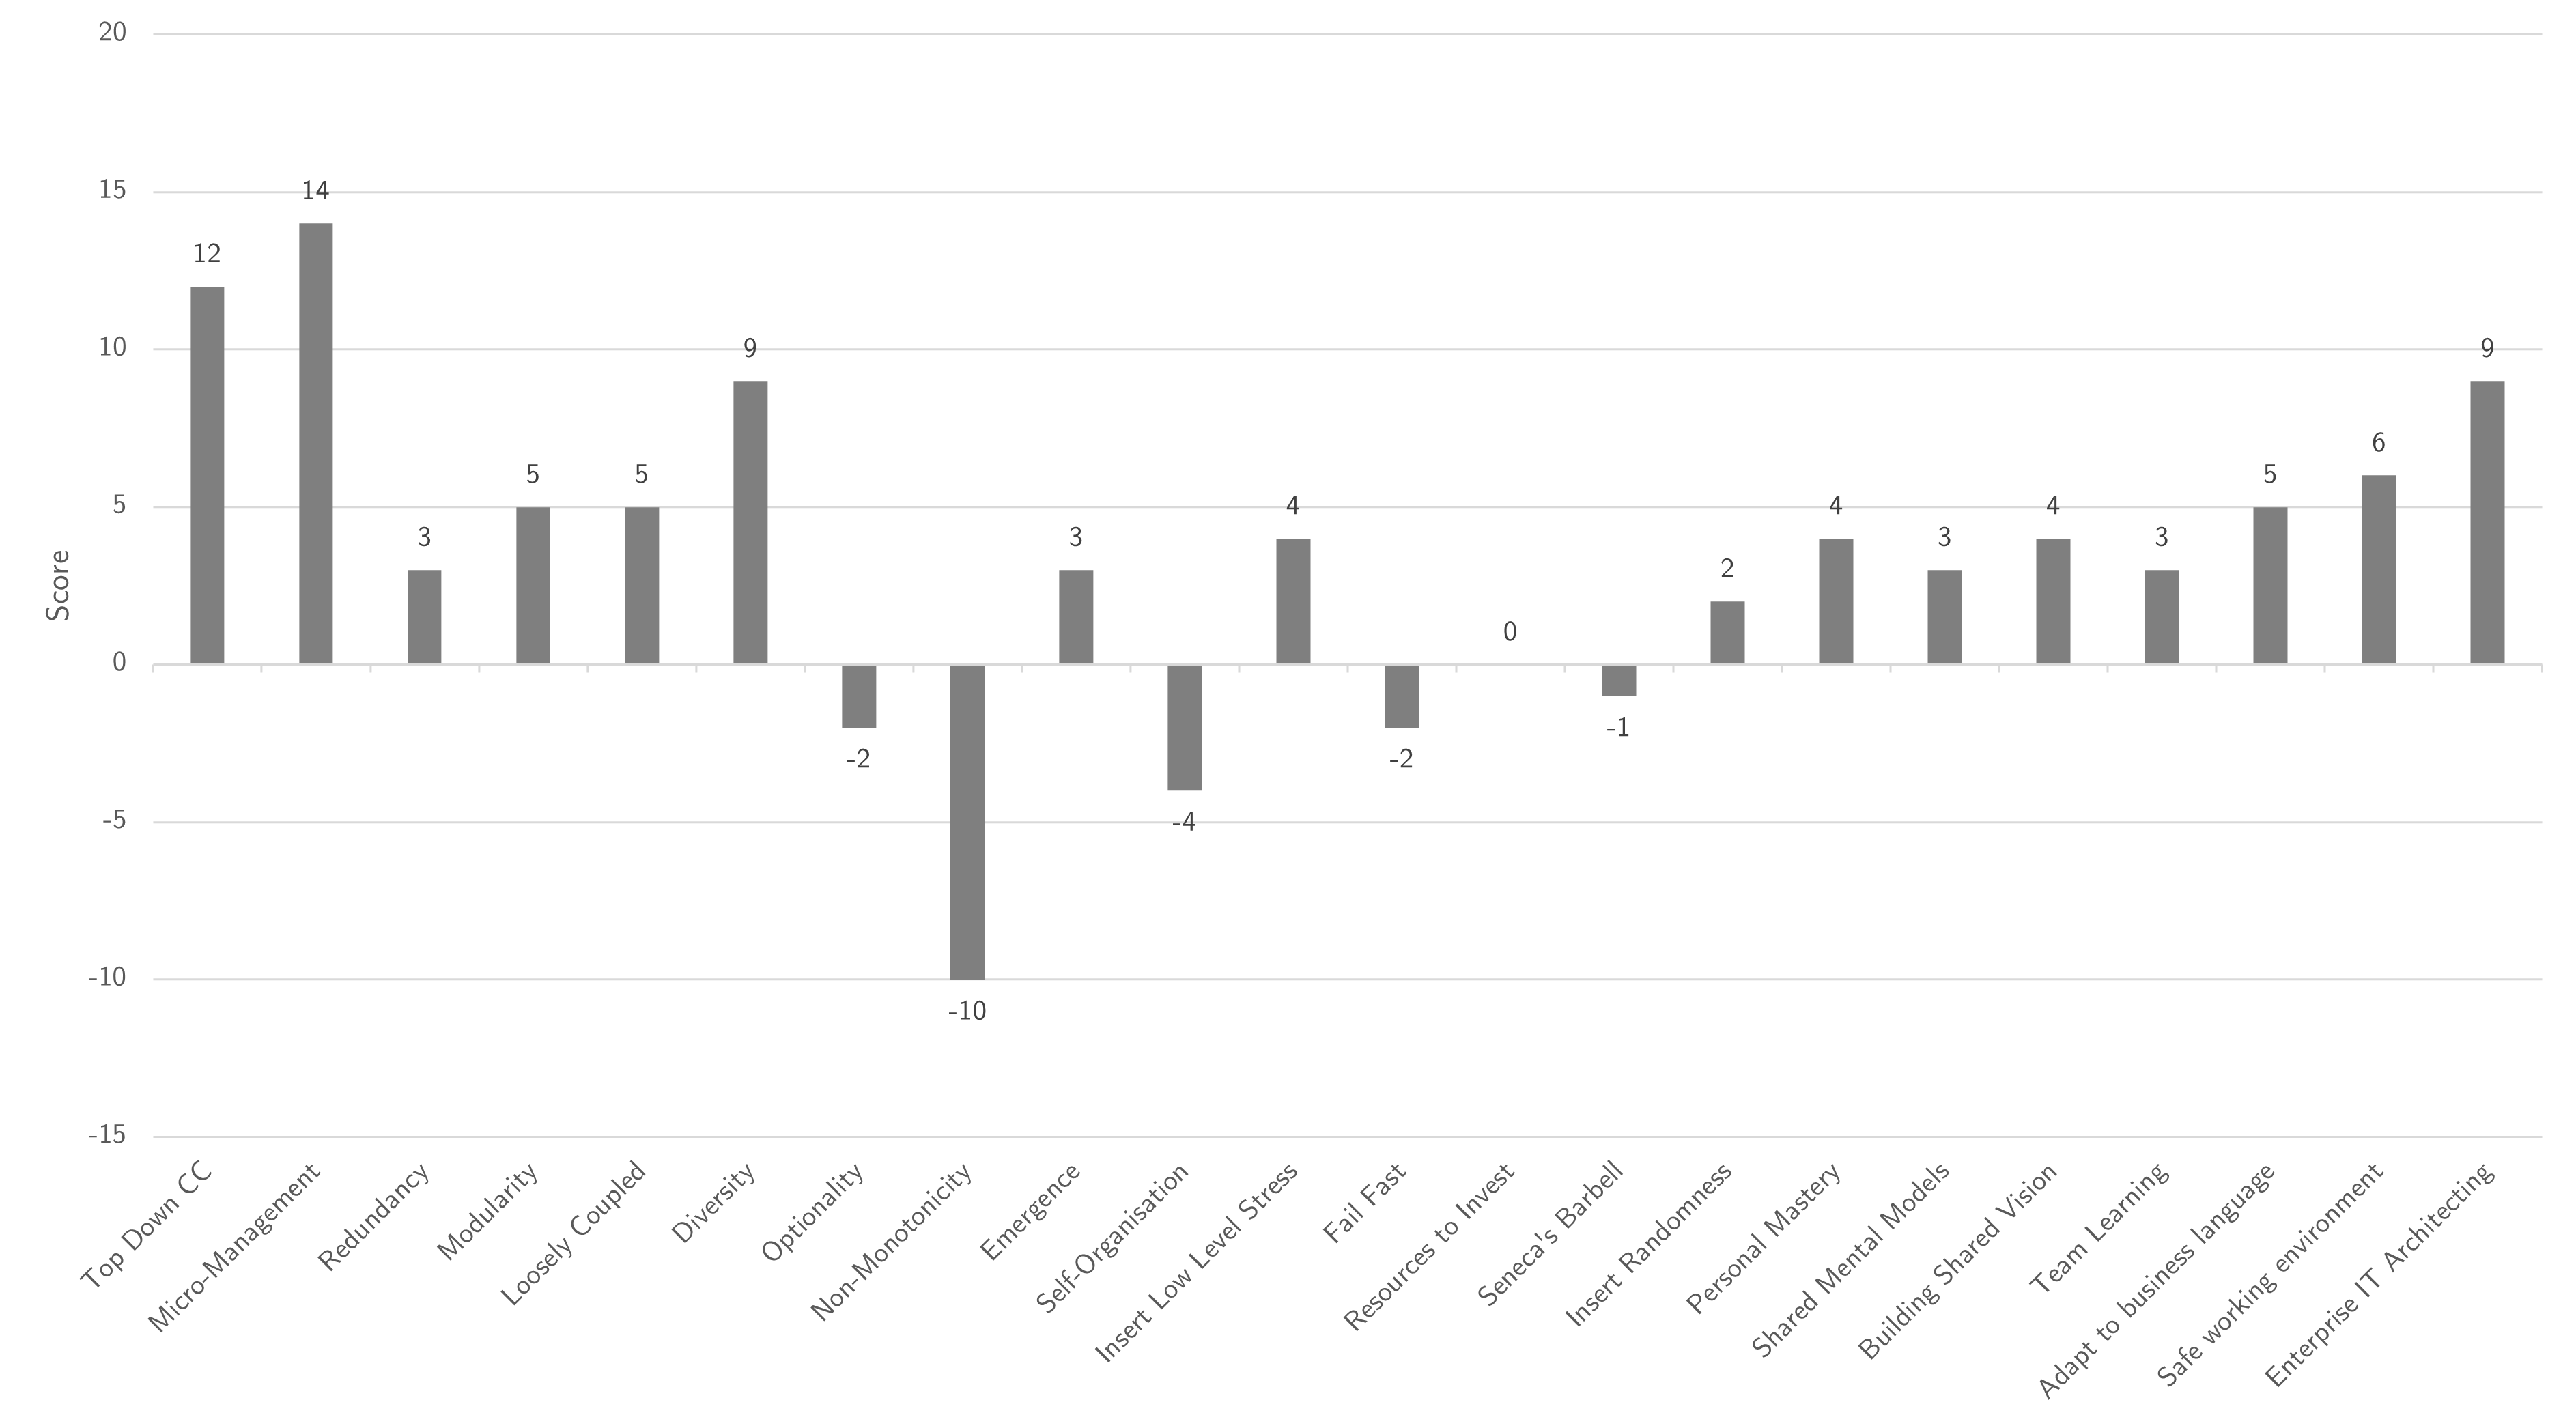
\includegraphics[width=\textwidth]{images/scoreofattributes}
	\caption[Score of attributes from interviews]{Score of attributes from interviews}
	\label{fig:scoreofattributes}
\end{figure}
The \acrshort{ea} school of thought is the last that needs interpretation. The questions on \acrshort{ea} were on \acrshort{ea} practices in the \gls{ps}. Currently, in the \gls{ps} the leading school of thought is \gls{enterpriseitarchitecting}. The \acrshort{ea} practise of the \gls{ps} must change to achieve \gls{antifragility} with \acrshort{ea}. \acrshort{ea} should foster the school of thought of \gls{enterpriseecologicaladaptation}. \Gls{enterpriseecologicaladaptation} is the school that has some certainty that it has a positive influence on achieving \gls{antifragility} in the \gls{ps}  (\cref{sec:tbenterprisearchitecture}).
\section{Attributes most likely to be a success factor}
\label{sec:attributeslikelysf}
The result of analysis of the interviews is the selection of fourteen attributes (\cref{tab:interviewpossiblesf}) that are possible attributes that have a positive influence on \acrlong{ea} in achieving \gls{antifragility} in the Dutch \gls{ps}. We replaced the Enterprise Architecture school of thought of Enterprise Ecological Adaptation with its \glspl{attribute}.
\begin{longtable}{@{}ll@{}}
	\toprule%
	\textbf{Attribute} & \textbf{Category}  \\%
	\midrule%
	\endhead%
	\hline
	\endfoot%
	\caption[Possible success factors identified from interviews]{Possible success factors identified from interviews}
	\label{tab:interviewpossiblesf}
	\endlastfoot%
	\Gls{optionality} & \Gls{amplifyvariety} \\%
	\Gls{nonmonotonicity} & \Gls{amplifyvariety} \\%
	\Gls{selforganisation} & \Gls{amplifyvariety} \\%
	\Gls{failfast} & \Gls{amplifyvariety} \\%
	\Gls{resourcestoinvest} & \Gls{amplifyvariety} \\%
	\Gls{senecabarbell} & \Gls{amplifyvariety} \\%
	\Gls{systeminenvironment} & \acrshort{ea} \Gls{enterpriseecologicaladaptation} \\%
	\Gls{holisticsystemicstance} & \acrshort{ea} \Gls{enterpriseecologicaladaptation} \\%
	\Gls{organisationallearning} & \acrshort{ea} \Gls{enterpriseecologicaladaptation} \\%
	\Gls{environmentallearning} & \acrshort{ea} \Gls{enterpriseecologicaladaptation} \\%
	\Gls{intraorganisationalcoherency} & \acrshort{ea} \Gls{enterpriseecologicaladaptation} \\%
	\Gls{systeminenvironmentcoevolutionlearning} & \acrshort{ea} \Gls{enterpriseecologicaladaptation} \\%
	\Gls{safeworkingenvironment} & New finding \\%
	\Gls{adapttobusinesslanguage} & New finding \\%
	\bottomrule%
\end{longtable}%
%This set of possible success factors was used as a proposal to the expert group for validation (\cref{ch:expertgroup}).